\section{Metodologia de Gestão de Projeto}

A seleção da metodologia ágil de gestão de projetos \textit{\gls{Kanban}} foi feita devido à sua notável capacidade de gerenciar eficazmente mudanças e incertezas ao longo do projeto. Com o intuito de promover a coesão, alinhamento e colaboração harmônica entre os membros da equipe, são empregadas ferramentas essenciais que garantem o pleno funcionamento do processo. As seguintes ferramentas desempenham papéis fundamentais nesse contexto:

Para viabilizar reuniões e discussões eficientes, a plataforma \textit{\gls{Discord}} é adotada como meio principal. Ela proporciona um ambiente virtual propício para a interação e troca de ideias entre os participantes do projeto. Através do \textit{\gls{Discord}}, é possível promover debates construtivos e manter a equipe atualizada sobre os progressos e desafios do projeto.

Com o propósito de agilizar a comunicação e facilitar a resolução imediata de dúvidas, o aplicativo \textit{\gls{Whatsapp}} é utilizado. Essa ferramenta se mostra valiosa para estabelecer conexões rápidas entre os membros da equipe, permitindo a rápida troca de informações e esclarecimentos pontuais.

Para a divulgação das atividades executadas e o compartilhamento de informações relevantes, o \textit{\gls{Blog}} assume um papel crucial. Essa plataforma online serve como um espaço dedicado à documentação das etapas cumpridas, permitindo que os membros da equipe acompanhem o desenvolvimento do projeto de forma transparente e estruturada.

O \textit{\gls{Jira}} é a plataforma eleita para a distribuição e controle das tarefas, como representado na figura \ref{Jira}. Esta ferramenta centraliza a atribuição de responsabilidades, facilitando o acompanhamento do status de cada atividade. O \textit{\gls{Jira}} não apenas contribui para a organização eficaz, mas também para a identificação de possíveis gargalos e atrasos, possibilitando ações corretivas oportunas.

\begin{figure}[H]
	\centering
	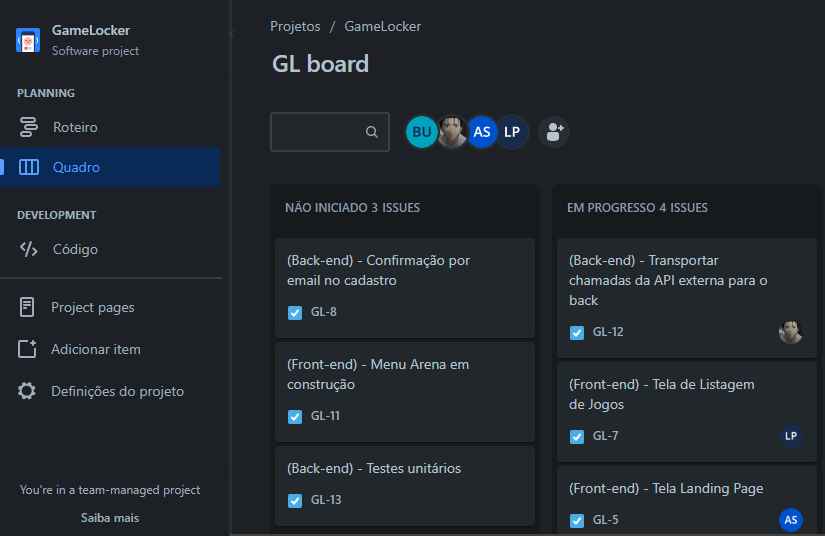
\includegraphics[scale=0.6]{imagens/planejamentoGerenciamento/jira.png}
	\caption{Jira}
	\label{Jira}
	\fonte{Autores}
\end{figure}

